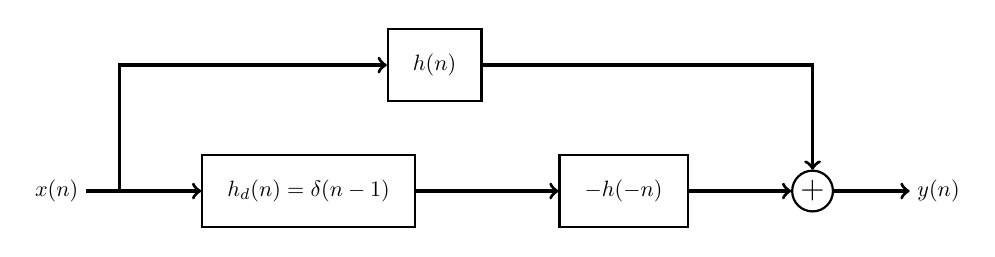
\begin{tikzpicture}[scale=0.8, transform shape]
    \node[circle,draw,thick,inner sep=0.05cm] (plus) at (0,0) {\Large +} ;
    \node[rectangle,draw,thick,inner sep=0.4cm] (minus_h_minus_n) at (-3,0) {$-h(-n)$} ;
    \node[rectangle,draw,thick,inner sep=0.4cm] (hd) at (-8,0) {$h_d(n)=\delta(n-1)$} ;
    \node[rectangle,draw,thick,inner sep=0.4cm] (h) at (-6,2) {$h(n)$} ;
    \node[xshift=-4cm] (x_n) at (hd) {$x(n)$} ;
    \node[xshift=-3cm,inner sep=-0.1] (x_n_arrow_cross) at (hd) {} ;

    \node[xshift=2cm] (y_n) at (plus) {$y(n)$} ;

    \draw[->, very thick] (x_n) -- (hd.west) ;
    \draw[->, very thick] (x_n_arrow_cross) |- (h.west) ;
    \draw[->, very thick] (h.east) -| (plus.north) ;
    \draw[->, very thick] (minus_h_minus_n.east) -- (plus.west) ;
    \draw[->, very thick] (hd.east) -- (minus_h_minus_n.west) ;
    \draw[->, very thick] (plus.east) -- (y_n.west) ;
\end{tikzpicture}